\chapter{Theory}
\label{ch:theory}

The hardware design and validation described in Chapter~\ref{ch:methods} rest on three theoretical foundations. Section~\ref{sec:human_physiology} covers the physiological systems used by \gls{emg} and \gls{eda} in this thesis. Sections~\ref{sec:EMG} and~\ref{sec:EDA} cover each modality, including the signal characteristics and measurement constraints that shape the circuit design. Section~\ref{sec:ground_loops} covers the ground loop problem that arises from co-locating the two measurement circuits.

\section{Physiological Background} \label{sec:human_physiology}

This section covers the three physiological systems relevant to the thesis. The nervous system controls both skeletal muscle activity and sweat gland activity (EDA signal). The skin is the measurement interface for both signals. Skeletal muscle is the source of the EMG signal.

\subsection{Human Nervous System} \label{sec:human_nervous_system}

The human nervous system is divided into two main parts: the central nervous system and the \gls{pns}~\cite{bazira_overview_2021}. This thesis concerns the \gls{pns} and its subdivisions, illustrated in Figure~\ref{fig:nervous_system_tree}.

The \gls{pns} is further divided into the somatic nervous system and the autonomic nervous system~\cite{bazira_overview_2021}. The somatic nervous system is responsible for controlling voluntary movements by transmitting motor commands to skeletal muscles~\cite{bazira_overview_2021, kamen_essentials_2010}. This is the nervous system branch involved in \gls{emg} measurements. The autonomic nervous system regulates involuntary bodily functions and is further divided into the sympathetic, parasympathetic, and enteric subdivisions~\cite{bazira_overview_2021}. The \gls{sns} is relevant to this thesis because it controls eccrine sweat gland activity, which is the basis of \gls{eda}~\cite{boucsein_electrodermal_2012, ellaway_sweat_2010, banganho_electrodermal_2022}. Section~\ref{sec:sweat} describes the structure and location of these glands.

\begin{figure}[!htbp]
    \centering
    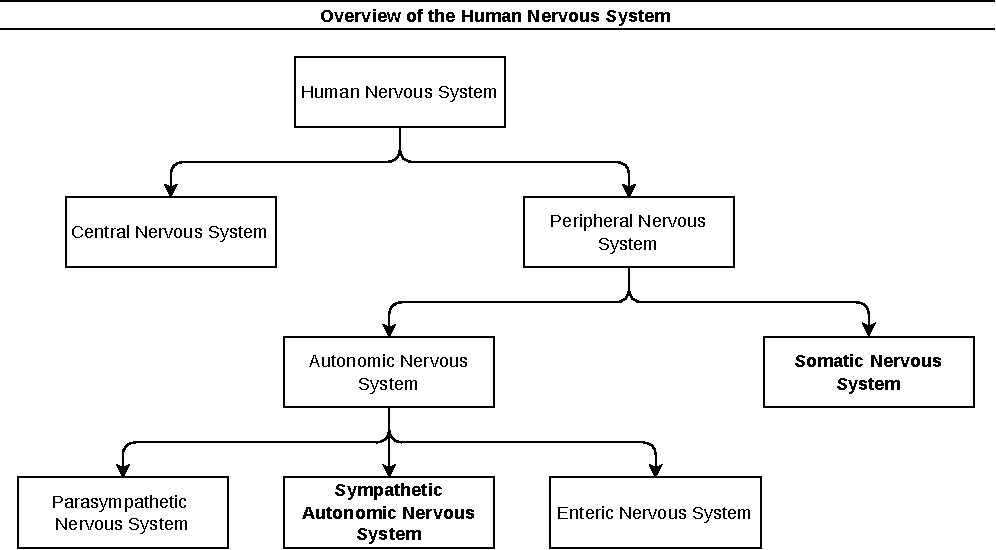
\includegraphics[width=0.8\textwidth]{figures/human_nervous_system.drawio (cropped) (pdfresizer.com).pdf}
    \caption{Overview of the human nervous system. Branches relevant to the thesis are bolded.}
    \label{fig:nervous_system_tree}
\end{figure}

\subsection{The Skin} \label{sec:skin}
EDA and surface EMG are acquired through electrodes placed on the skin surface. The structural and electrical properties of the skin, therefore, directly affect the measured signals.

\subsubsection{Skin Structure} \label{sec:skin_structure}
The skin is composed of three layers: the epidermis, the dermis, and the hypodermis~\cite{lopez-ojeda_anatomy_2025}. Figure~\ref{fig:skin_layers} illustrates these layers and the underlying muscle tissue. The epidermis is the outermost layer, with a thickness that ranges from \SIrange{50}{200}{\micro\metre} at most body sites but reaches approximately \SI{1}{\milli\metre} at the palms and soles~\cite{boucsein_electrodermal_2012}. The stratum corneum is the outermost sublayer of the epidermis and consists of dead cells with low moisture content~\cite{banganho_electrodermal_2022}. The dermis lies beneath the epidermis, is much thicker, and contains sweat glands and blood vessels~\cite{boucsein_electrodermal_2012, banganho_electrodermal_2022}. The hypodermis is the deepest layer and connects the skin to the underlying muscle tissue.

\begin{figure}[!htbp]
    \centering
    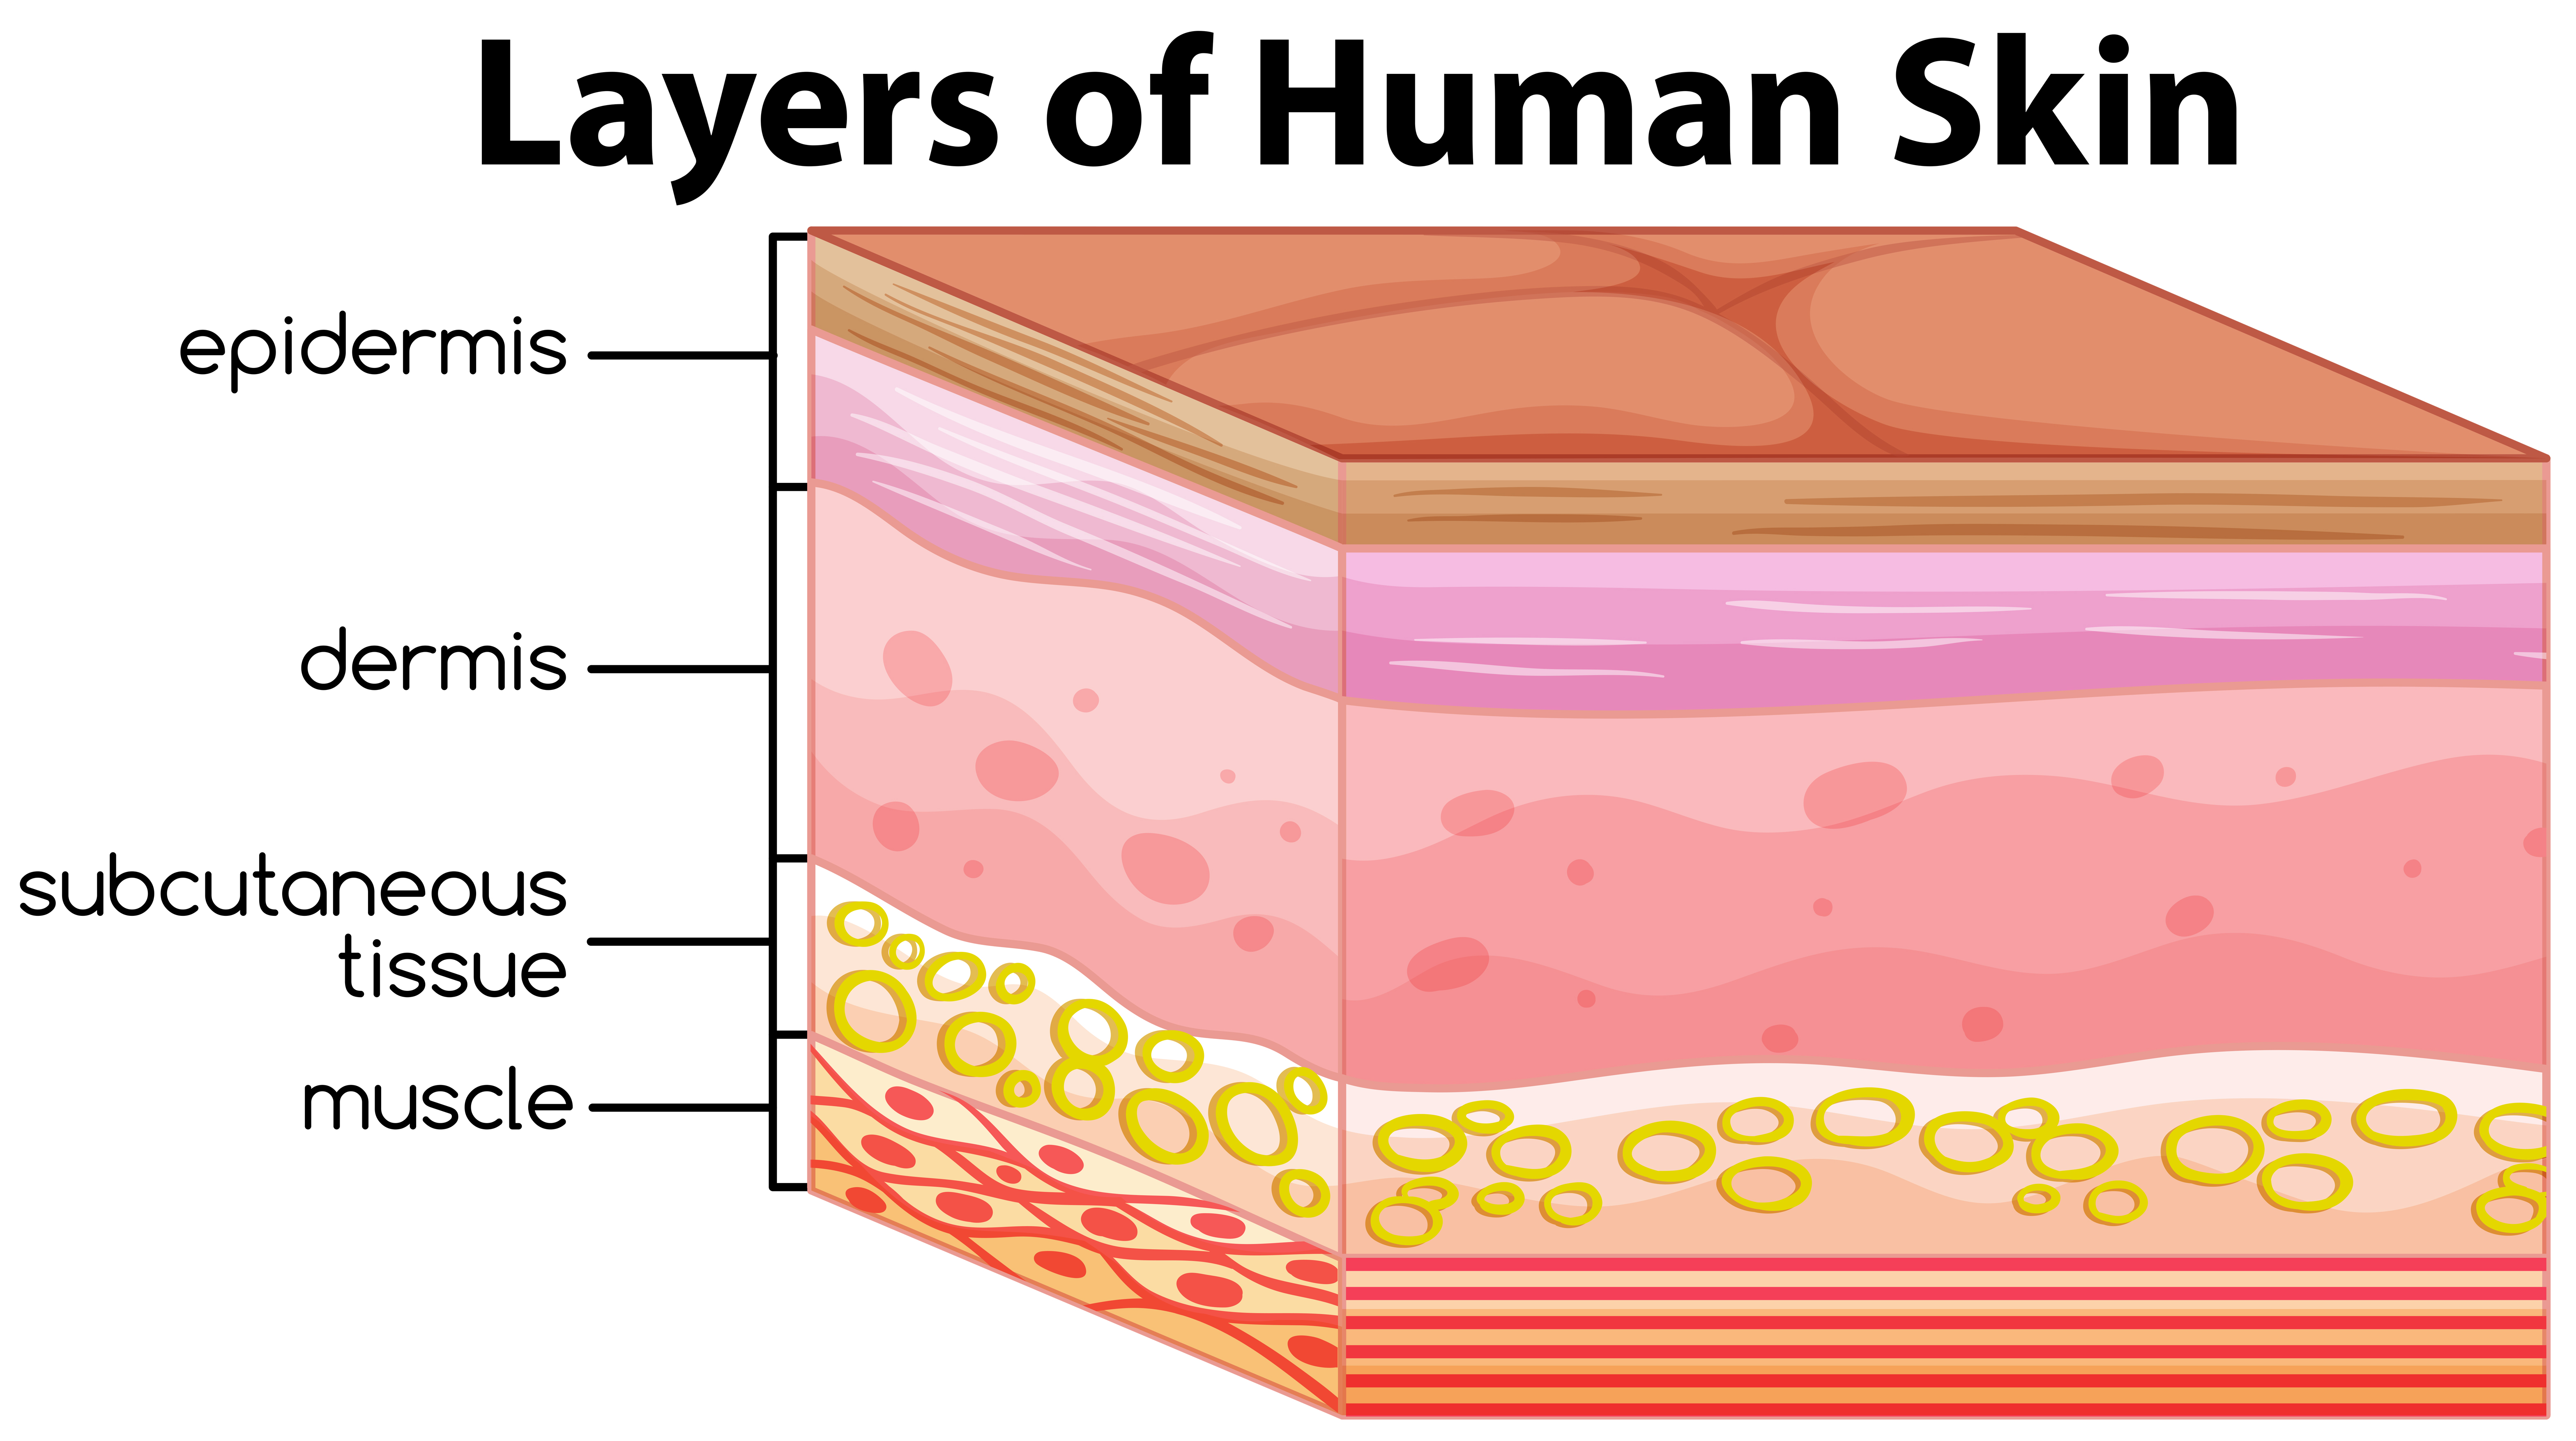
\includegraphics[width=0.55\textwidth]{figures/skin_layer.jpg}
    \caption{Layered structure of the skin, showing the epidermis, dermis, hypodermis (subcutaneous tissue), and underlying muscle. Image from \href{https://www.vecteezy.com/vector-art/445514-layers-of-human-skin-concept}{https://www.vecteezy.com/vector-art/445514-layers-of-human-skin-concept}.}
    \label{fig:skin_layers}
\end{figure}

\subsubsection{Sweat Glands \& Sweat Ducts} \label{sec:sweat}
The eccrine sweat glands introduced in Section~\ref{sec:human_nervous_system} are one of two types of sweat glands. The other type is apocrine~\cite{cacioppo_handbook_2007}. The apocrine glands are found mainly in the axillae and genitals and contribute little to overall sweating~\cite{boucsein_electrodermal_2012}. The eccrine glands are distributed across most of the body. Each gland sits in the hypodermis or dermis and connects to the skin surface through a narrow duct that passes through the dermis and the epidermis~\cite{boucsein_electrodermal_2012}, as shown in Figure~\ref{fig:sweat_glands}. When the gland activates, sweat fills the duct. Because sweat contains ions, the filled duct acts as a low-resistance pathway through the stratum corneum~\cite{tronstad_current_2022}. The palmar and plantar regions have higher densities of eccrine glands and are more responsive to emotional stimuli than the trunk and limbs~\cite{tronstad_current_2022, boucsein_electrodermal_2012}. These sweating dynamics determine the electrical behavior of the skin at the measurement site.

\begin{figure}[!htbp]
    \centering
    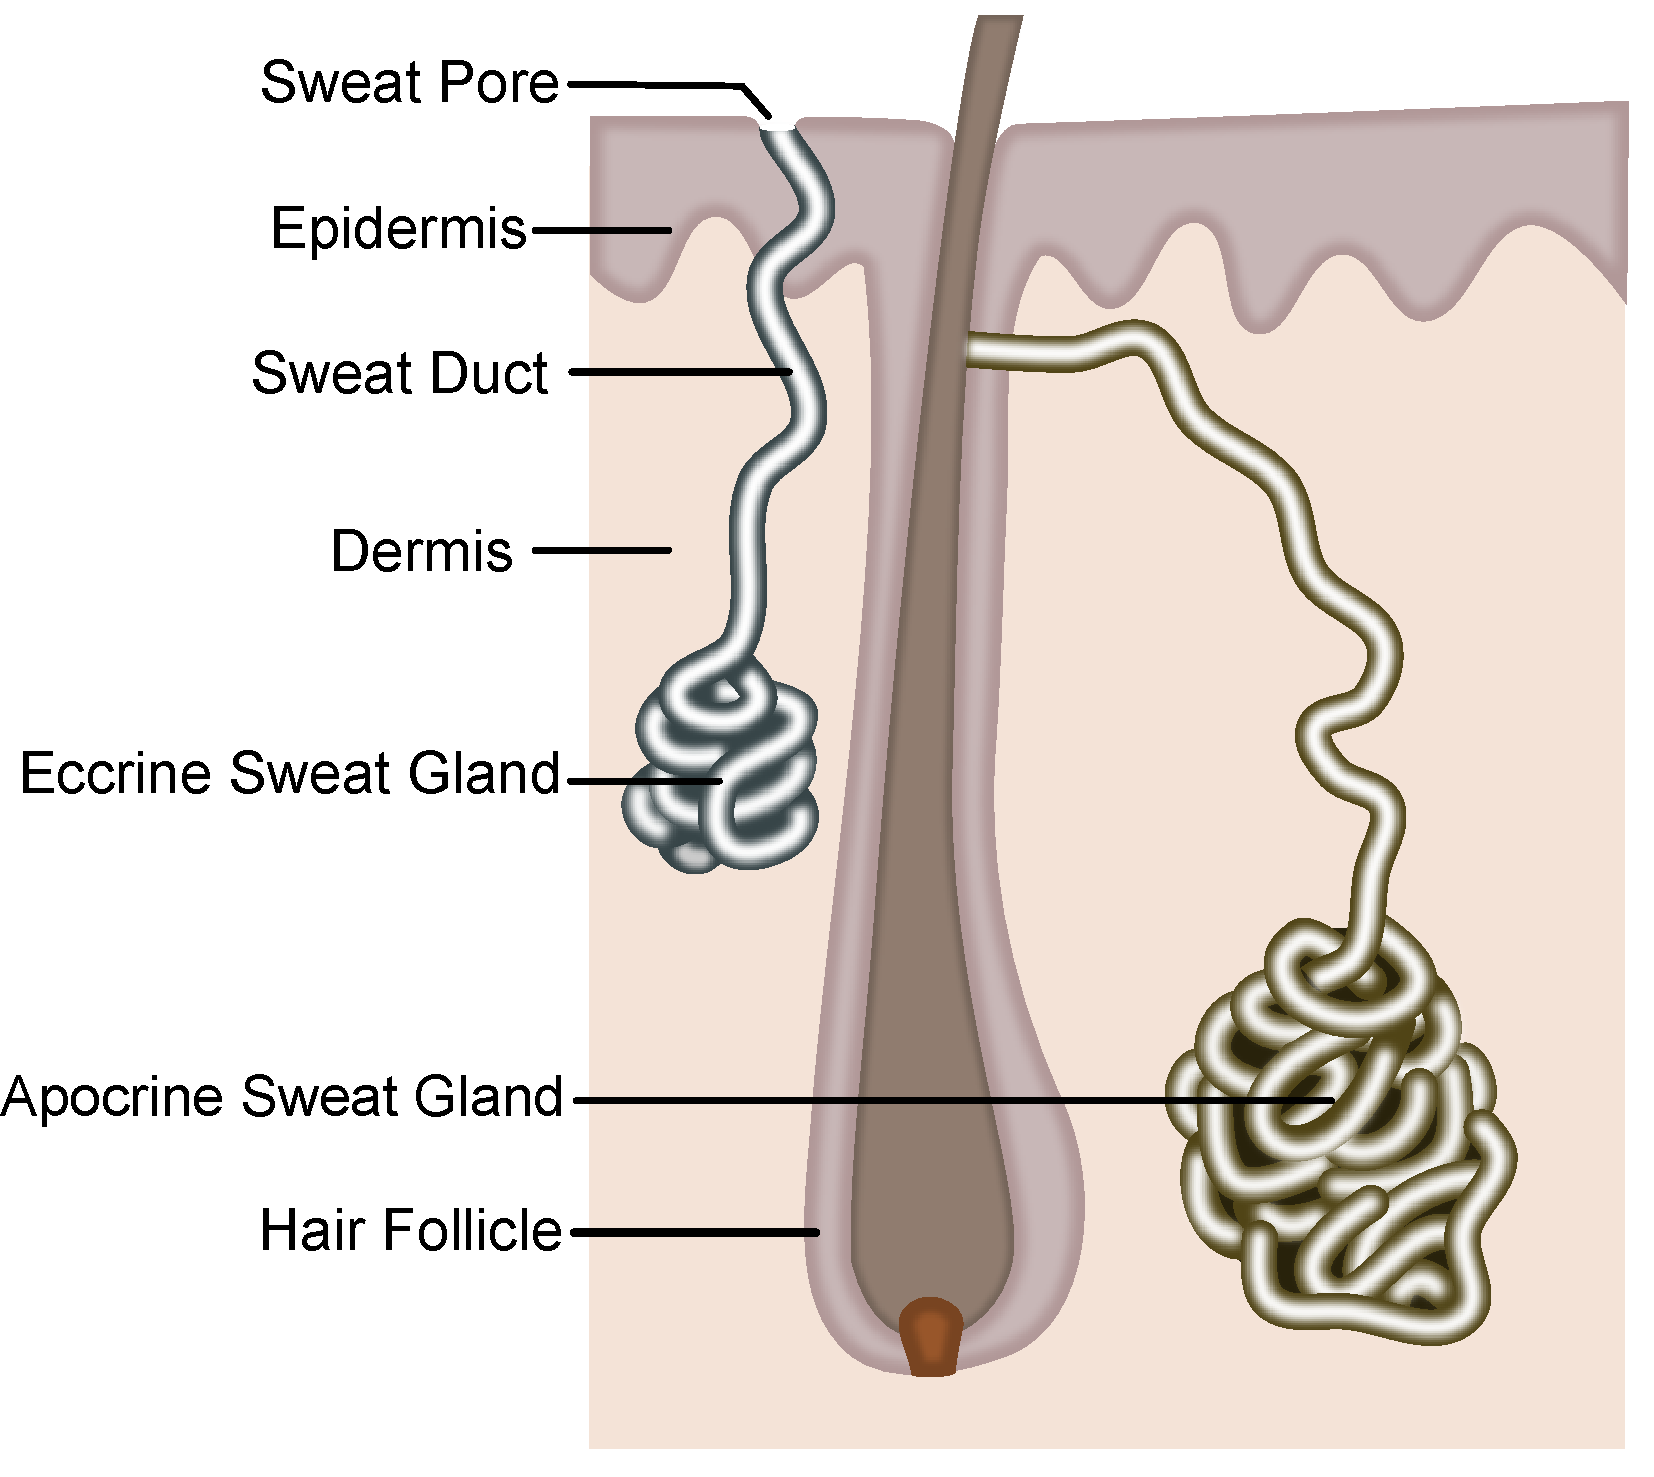
\includegraphics[width=0.45\textwidth]{figures/sweat_glands.pdf}
    \caption{Cross-section of skin showing an apocrine sweat gland, an eccrine sweat gland, and their ducts opening at the skin surface. A hair follicle is shown for anatomical context. Adapted from Glafoululle des Alpes (2022), \textit{Skin Glandes}, \href{https://commons.wikimedia.org/wiki/File:Skin_Glandes_-_FR.svg}{https://commons.wikimedia.org/wiki/File:Skin\_Glandes\_-\_FR.svg}, CC BY-SA 4.0.}
    \label{fig:sweat_glands}
\end{figure}

\FloatBarrier

\subsubsection{Electrical Properties} \label{sec:human_el_properties}
The stratum corneum has high electrical impedance because of its low moisture content and dense structure~\cite{tronstad_current_2022}. Two distinct pathways alter this impedance during sweating. When eccrine sweat ducts fill, the ionic content of the sweat forms a low-resistance pathway through the stratum corneum and contributes to the phasic \gls{scr}~\cite{tronstad_current_2022}. Continued sweating also hydrates the stratum corneum itself and raises its bulk conductivity, which underlies the tonic \gls{scl}~\cite{boucsein_electrodermal_2012}. The two pathways act together to shape the recorded skin conductance signal.

The impedance at the electrode-skin interface affects both EDA and EMG recordings. For EMG, high electrode-skin impedance reduces the signal amplitude at the amplifier input and can worsen \gls{cmrr}~\cite{kamen_essentials_2010}. For EDA, it increases the total impedance along the measurement path and reduces sensitivity to conductance changes caused by sweat activity.

\subsubsection{Skin Preparation} \label{sec:skin_prep}
EMG and EDA have opposing skin preparation requirements. EMG recordings benefit from low electrode-skin impedance, so the skin is typically cleaned with alcohol and lightly abraded to remove dead cells from the stratum corneum~\cite{kamen_essentials_2010, konrad_abc_2006}. Exosomatic EDA recordings rely on the stratum corneum itself as the high-impedance layer through which sweat ducts produce the conductance changes of interest. Abrasion is therefore not recommended for EDA, as it lowers baseline impedance and reduces the relative contribution of sweat duct activity to the signal~\cite{boucsein_electrodermal_2012}.


\subsection{Skeletal Muscle}\label{sec:muscle}
%Mention that muscle tissue is anisotropic - Ørjan sin bok
Skeletal muscle consists of bundles of muscle fibers~\cite{mukund_skeletal_2020}. Each fiber is a long, cylindrical cell with an excitable membrane that generates electrical signals~\cite{kamen_essentials_2010}. Motoneurons innervate these muscle fibers. A single motoneuron and all of the fibers it innervates together form a \gls{mu}~\cite{whittaker_fundamentals_2012, konrad_abc_2006}, illustrated in Figure~\ref{fig:motor_unit}. The \gls{mu} is the smallest unit of muscle activation. When the motoneuron fires, all of its fibers contract simultaneously. The electrical and functional properties of \glspl{mu} are discussed in Section~\ref{sec:EMG_signal}.

\begin{figure}[!htbp]
    \centering
    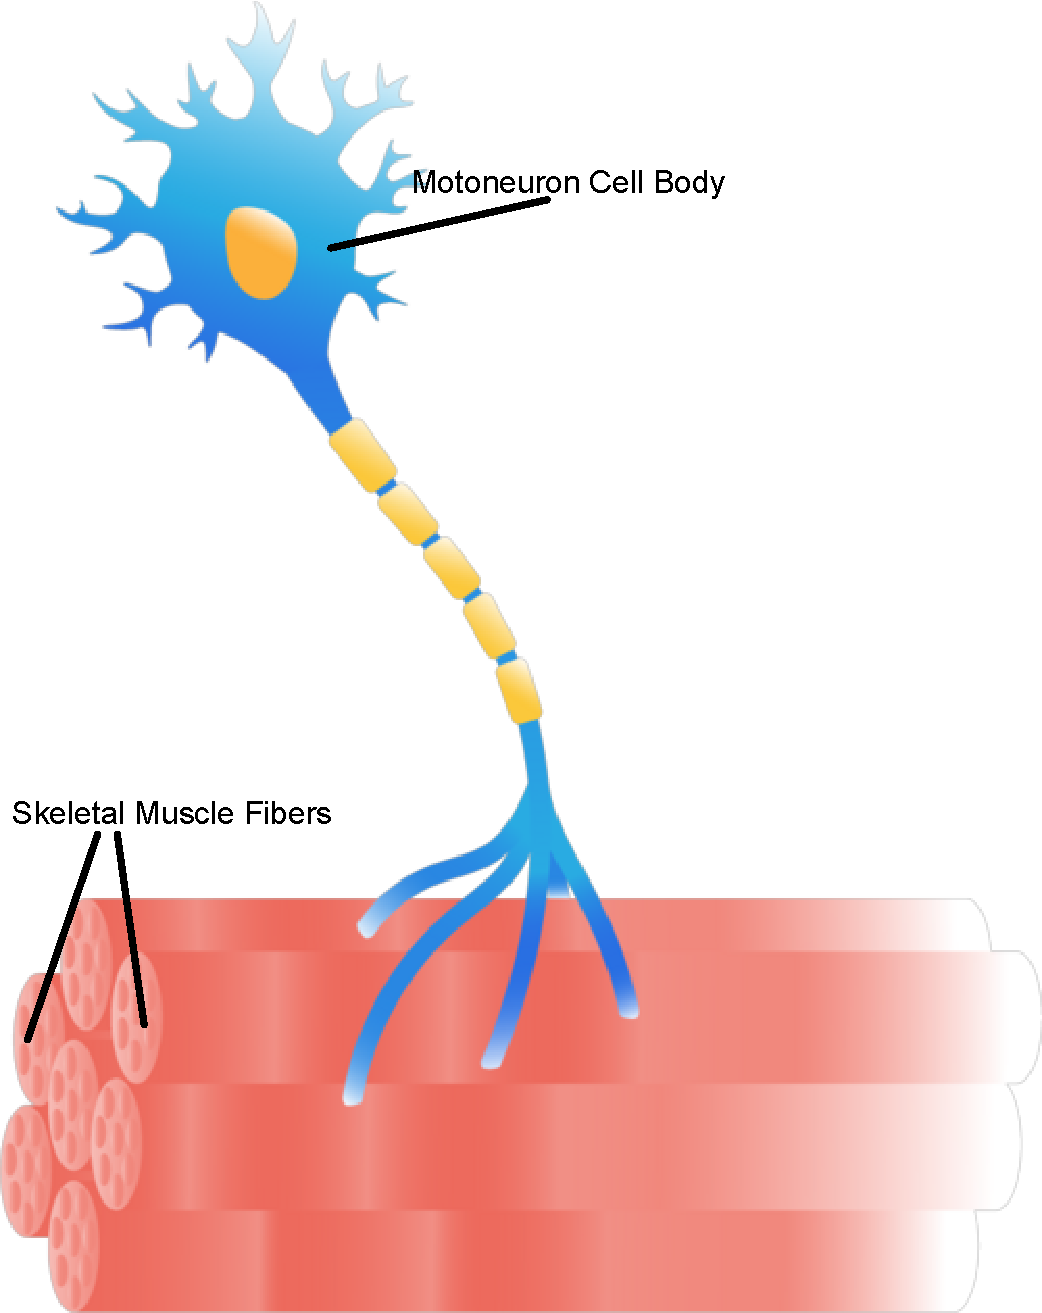
\includegraphics[width=0.5\textwidth]{figures/Motor_Unit.pdf}
    \caption{Schematic of a motor unit: one motoneuron innervating a bundle of skeletal muscle fibers. Adapted from ScholarJay (2022), \textit{Motor Unit}, \href{https://commons.wikimedia.org/wiki/File:Motor_Unit.png}{https://commons.wikimedia.org/wiki/File:Motor\_Unit.png}, CC BY-SA 4.0.}
    \label{fig:motor_unit}
\end{figure}

Muscle tissue is anisotropic, with higher electrical conductivity along the fibers than across them~\cite{kamen_essentials_2010, grimnes_bioimpedance_2015}. The tissue layers between the muscle and the skin surface act as a volume conductor with low-pass filtering properties. This filtering reduces the amplitude of higher-frequency components before they reach the skin surface~\cite{kamen_essentials_2010, konrad_abc_2006}. Both characteristics affect electrode placement and the signal characteristics in surface \gls{emg}, as discussed in Section~\ref{sec:EMG_measurement}.

\FloatBarrier

\section{Electromyography} \label{sec:EMG}
\Gls{emg} records the electrical activity produced by skeletal muscles~\cite{chowdhury_surface_2013}. Clinical neurophysiology uses \gls{emg} to assess muscle activation and to diagnose neuromuscular disorders~\cite{kamen_essentials_2010, whittaker_fundamentals_2012, alcan_current_2023}. This thesis uses \gls{emg} in a non-diagnostic context: to measure muscle activation together with \gls{eda} at the same electrode site. The design of the acquisition front-end, therefore, depends on understanding both the origin of the \gls{emg} signal and the practical trade-offs of the available recording techniques.

Section~\ref{sec:EMG_signal} describes the physiological origin of the \gls{emg} signal. Section~\ref{sec:EMG_measurement} then covers the two main recording techniques: intramuscular \gls{emg} in Section~\ref{sec:Intra_EMG} and \gls{semg} in Section~\ref{sec:sEMG}. The technique used in this thesis is \gls{semg}, and its signal structure, electrode configuration, and noise sources are described in the final subsections.

\subsection{Physiological Basis and Signal Origin} \label{sec:EMG_signal}
% Section pipeline: Bioelectric framing → Cellular mechanism → From fiber to measurable unit → Amplitude regulation → Frequency content → Statistical character + section hand-off.
% Chapter role: Supplies the signal-property premises that methods use for RMS over mean (stochastic + zero-mean), contraction RMS as activation index (amplitude scaling), and electrode alignment parallel to fibers (dipole propagation).

% Bioelectric framing
\Gls{emg} passively records bioelectricity, the endogenous electrical potentials generated within biological tissues~\cite{grimnes_bioimpedance_2015}. In this thesis, the bioelectric sources are skeletal muscle fibers. The physiological processes that generate the signal set the amplitude and frequency content seen at the electrode.

% Cellular mechanism
% Don't include alpha motoneuron - AI USE
As described in Section~\ref{sec:muscle}, skeletal muscle is organized into \glspl{mu}. A \gls{mu} consists of a single motoneuron and all the muscle fibers it innervates~\cite{konrad_abc_2006}. When the motoneuron fires, all innervated fibers generate action potentials almost simultaneously~\cite{kamen_essentials_2010}. Each \gls{mfap} arises from a depolarization-repolarization cycle at the fiber membrane. The result is a traveling depolarization zone, or electrical dipole, that propagates along the fiber at a conduction velocity of \SIrange{2}{6}{\meter\per\second}~\cite{konrad_abc_2006}. Each active fiber, therefore, contributes a short-lived dipole to the electric field at the skin.

% From fiber to measurable unit
The dipoles from fibers belonging to the same \gls{mu} sum into a single compound waveform. This waveform is the \gls{muap}, shown in Figure~\ref{fig:muap}. The \gls{muap} is the smallest unit of muscle activity that can be detected at the skin with surface electrodes and a suitable amplifier~\cite{kamen_essentials_2010}. It is therefore the basic building block of the recorded \gls{emg} signal.

\begin{figure}[!htbp]
    \centering
    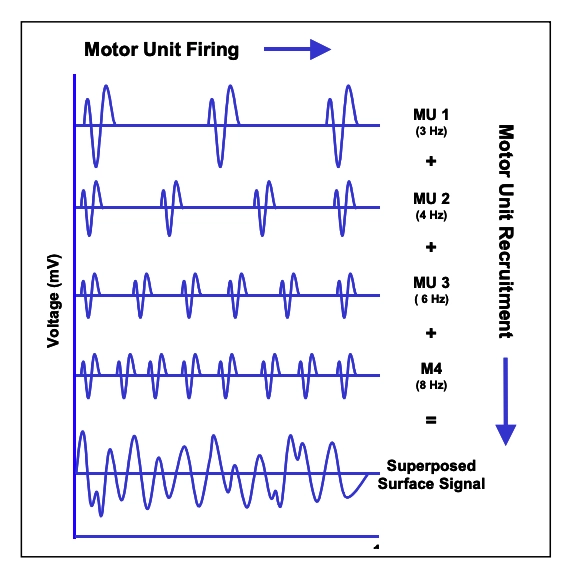
\includegraphics[width=0.6\textwidth]{figures/MUAP_superposition.png}
    \caption{Individual MFAPs summing into a MUAP. Reproduced from~\textcite{konrad_abc_2006} with permission.}
    \label{fig:muap}
\end{figure}

% Amplitude regulation
The magnitude and temporal density of the \gls{emg} signal reflect how the nervous system regulates muscular force~\cite{kamen_essentials_2010}. Two mechanisms apply: recruitment of additional \glspl{mu} and modulation of their firing rates. \Glspl{mu} are recruited from smallest to largest, so units with fewer or smaller fibers fire first as force demand increases~\cite{cavalcanti_garcia_surface_2010}. As contraction intensity rises, more \glspl{mu} are recruited, and their firing rates increase. The result is a higher density of overlapping \glspl{muap} at the skin. The signal amplitude, therefore, scales with contraction intensity, making \gls{emg} amplitude an established index of muscle activation. The relationship between \gls{emg} amplitude and mechanical force is not strictly linear and depends on factors such as muscle length, fatigue, and electrode placement~\cite{duchateau_distribution_2022, kamen_essentials_2010}.

% Frequency content
The frequency content of the \gls{emg} signal carries physiological information beyond amplitude. Spectral shape depends on muscle fiber conduction velocity and on changes associated with muscle fatigue~\cite{kamen_essentials_2010, cavalcanti_garcia_surface_2010}. Volume conduction through the tissue between the fibers and the skin surface reduces the amplitude of higher-frequency components, as discussed further in Section~\ref{sec:sEMG_signal}.

% Statistical character + section hand-off
The active \glspl{mu} and their firing times continuously change, so the \gls{semg} signal recorded at the skin is stochastic and its exact waveform cannot be predicted or reproduced~\cite{konrad_abc_2006}. The signal is biphasic, with approximately symmetric positive and negative amplitudes and a mean near zero. At low contraction levels, individual \glspl{muap} may still be distinguishable, but as intensity increases, they merge into a dense waveform known as an interference pattern~\cite{konrad_abc_2006, cavalcanti_garcia_surface_2010}. The \gls{semg} therefore provides a global measure of muscle activation but cannot resolve the activity of individual \glspl{mu}~\cite{cavalcanti_garcia_surface_2010}. The stochastic, zero-mean character of the signal shapes the amplitude and spectral measures used later in this thesis, and it sets the starting point for the recording techniques described in Section~\ref{sec:EMG_measurement}.

\FloatBarrier

\subsection{Measurement Techniques} \label{sec:EMG_measurement}
% Two measurement techniques
Two main techniques are used to record \gls{emg}~\cite{kamen_essentials_2010}. Surface \gls{emg} uses electrodes placed on the skin over the target muscle. Intramuscular \gls{emg} uses needle or wire electrodes inserted into the muscle tissue. The two approaches differ in invasiveness, spatial scale, and the information they extract.

\subsubsection{Intramuscular EMG} \label{sec:Intra_EMG}
% Section pipeline: Physical setup and spatial selectivity → Spatial selectivity advantage → Practical limitations → Thesis-specific incompatibility with EDA.
% Chapter role: Rules out intramuscular EMG for this thesis on two grounds (practical limits + EDA co-location incompatibility), justifying the methods chapter's use of sEMG without further argument.

% Physical setup and spatial selectivity
%Invasive EMG
Intramuscular \gls{emg} involves inserting either a rigid concentric needle electrode or a fine flexible wire electrode through the skin and into the muscle belly. The recording surface of the electrode targets a small volume of tissue, usually just a few cubic millimeters, which allows the signal to reflect the summed activity of only a small number of \glspl{mu} in the immediate vicinity of the electrode tip~\cite{kamen_essentials_2010, karacan_comparison_2025}.

% Spatial selectivity advantage
This spatial selectivity is the main advantage of the technique, as it enables the identification of individual \glspl{muap} in the recorded trace~\cite{kamen_essentials_2010}. Multi-unit recording is particularly useful for examining deep or small muscles, and allows researchers to study \gls{mu} recruitment and firing rates~\cite{karacan_comparison_2025}. Single-unit recording is suited to investigate how individual \glspl{mu} respond to stimulation~\cite{karacan_comparison_2025}.

% Practical limitations
The cost of this resolution is invasiveness. Inserting electrodes through the skin causes discomfort and carries risks such as bleeding and infection~\cite{whittaker_fundamentals_2012, karacan_comparison_2025}. These risks limit the use of intramuscular \gls{emg} to clinical and laboratory settings under medical supervision.

% Thesis-specific incompatibility with EDA
For this thesis, an additional constraint arises from the need to record \gls{eda} simultaneously from the same skin site. \Gls{eda} is based on changes in the electrical properties of the skin (see Section~\ref{sec:EDA}). Any electrode penetrating the skin disrupts the electrodermal signal and damages the tissue on which the \gls{eda} sensor relies~\cite{boucsein_electrodermal_2012}. Intramuscular recording is therefore incompatible with simultaneous \gls{eda} measurement, leaving surface \gls{emg} as the only viable recording modality for this thesis.


\subsubsection{Surface EMG} \label{sec:sEMG}
% Section pipeline: Advantages and limitations → signal structure (amplitude + frequency) → electrode configuration (overview → definitions → terminology → functions → noise handling → specifications → placement) → noise sources (power-line → motion → crosstalk) → hand-off to methods.
% Chapter role: Supplies the signal specifications and design rationale (amplitude range, frequency bands, CMRR threshold, input impedance, electrode geometry, noise sources) that the methods chapter inherits when specifying the EMG acquisition hardware.

% Advantages and limitations of surface EMG
%Surface EMG
Surface electromyography (\gls{semg}) involves placing electrodes on the skin over a target muscle, leaving the underlying tissue intact. \Gls{semg} is noninvasive, does not require medical supervision, and allows the electrode site to share the skin with other electrode-based measurements such as \gls{eda}~\cite{konrad_abc_2006}. The technique has two main limitations. It works best for superficial muscles that are large enough to accommodate the recording electrodes. Its spatial resolution is lower than intramuscular recording~\cite{kamen_essentials_2010}.


\paragraph{sEMG Signal Structure} \label{sec:sEMG_signal}

% sEMG signal structure: amplitude and frequency
% Figure added
The raw \gls{semg} signal amplitude at the skin surface spans \SIrange{10}{5000}{\micro\volt}. During active contraction the amplitude is \SIrange{60}{300}{\micro\volt}, and at rest it falls to \SIrange{20}{30}{\micro\volt}~\cite{li_wearable_2021}, as shown in Figure~\ref{fig:raw_semg}. The frequency content spans \SIrange{10}{500}{\hertz}~\cite{yang_detection_2020, kamen_essentials_2010}, with most of the signal power concentrated between \SIrange{20}{150}{\hertz}~\cite{konrad_abc_2006}. The intervening tissue layers reduce the amplitude of higher-frequency components relative to intramuscular recordings~\cite{konrad_abc_2006, kamen_essentials_2010}.

% sEMG focus justified in Section 2.2.2.1

\begin{figure}[!htbp]
    \centering
    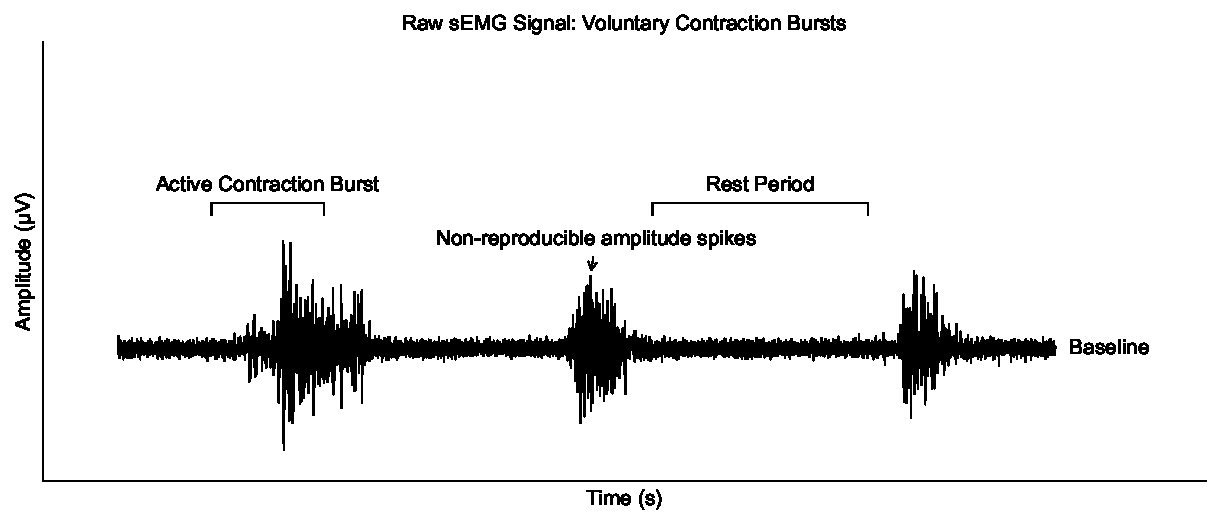
\includegraphics[width=0.9\textwidth]{figures/raw_semg_illustration.pdf}
     \caption{Illustrative composite of three voluntary contraction bursts recorded from the thumb muscles in this thesis. Each burst is followed by a rest period at baseline. The inter-burst intervals are shortened for display. The original recording used a \qty{15}{\second} inter-stimulus interval.}
    \label{fig:raw_semg}
\end{figure}

\FloatBarrier
% In monopolar config, is the ref electrode the same as the gnd electrode?
\paragraph{sEMG Electrode Configuration} \label{sec:sEMG_electrodes}

% Electrode configuration overview
Electrode configuration for \gls{semg} specifies the number of active recording surfaces and their arrangement relative to the muscle. The two most common configurations are monopolar and bipolar~\cite{kamen_essentials_2010}.

% Monopolar and bipolar definitions
In a monopolar configuration, a single active electrode is placed over the muscle. The potential is measured relative to a reference electrode placed on electrically inactive tissue such as a bony prominence~\cite{kamen_essentials_2010}. In a bipolar configuration, two active electrodes are placed over the muscle. The amplifier measures the potential difference between them, with a separate ground electrode on inactive tissue~\cite{kamen_essentials_2010, beck_comparison_2007}.

% Reference vs ground electrode terminology
%Talk about the reference electrode
In both monopolar and bipolar configurations, an electrode placed on electrically inactive tissue is essential. In monopolar recording, this electrode is called the reference electrode. In bipolar recording, it is called the ground electrode. The two terms denote different roles in the amplifier circuit but are often used interchangeably in the \gls{emg} literature~\cite{kamen_essentials_2010}.

% Electrical functions of the reference/ground electrode
Regardless of the terminology, this electrode serves three electrical functions. First, it establishes a stable zero-potential reference, since all voltages must be measured relative to a defined reference point. Second, it provides a low-impedance path for common-mode currents, which allows the differential amplifier to reject mains-frequency interference~\cite{kamen_essentials_2010}. Third, it serves as the return path for the amplifier's input bias current. Without this connection, the bias current has no path to flow. The amplifier inputs drift toward the supply rails, and the output saturates~\cite{noauthor_ina828_nodate}.

% Monopolar vs bipolar noise handling
%Difference between Monopolar and Bipolar recording
The key difference between the two configurations lies in how they handle noise. The monopolar technique captures the full signal at the active electrode. With only one electrode over the muscle, it is vulnerable to far-field interference that cannot be canceled out~\cite{beck_comparison_2007}. The bipolar configuration addresses this through differential amplification. Because both active electrodes sit close together over the same muscle, interference signals arrive at each electrode with nearly equal amplitude and phase. The amplifier subtracts one active input from the other, while the ground electrode establishes the common reference for both inputs. This common-mode rejection cancels the shared interference and amplifies only the difference, which carries the locally generated \gls{emg} signal. A side effect is that common-mode rejection also removes a small portion of the \gls{emg} signal itself, so the bipolar recording does not contain every detail available at the muscle~\cite{beck_comparison_2007}. Bipolar is the standard choice for \gls{semg} because the noise rejection it provides is essential, given the small signal amplitude.

% CMRR specification
The effectiveness of common-mode rejection is measured by the \gls{cmrr}, defined as the ratio of differential gain to common-mode gain. A \gls{cmrr} greater than \qty{95}{\decibel} is recommended for clinical and research \gls{semg} recordings~\cite{konrad_abc_2006}. For controlled isometric recordings, \qty{80}{\decibel} is reported as sufficient~\cite{kamen_essentials_2010}.

% Input impedance requirement
The amplifier input impedance should be at least 10 times the electrode-skin impedance to prevent loading the signal source. A recommended range is \SIrange{1}{10}{\mega\ohm}~\cite{konrad_abc_2006}.

% Electrode placement: inter-electrode distance and fiber alignment
Correct electrode placement is essential in bipolar recordings. The recommended inter-electrode distance is \qty{20}{\milli\meter} for large muscle bellies~\cite{konrad_abc_2006}. Smaller muscles require tighter spacing to keep both electrodes over the target tissue, as discussed in the methods chapter (Section~\ref{sec:electrode_placement}). Because muscle tissue is anisotropic (Section~\ref{sec:muscle}), the two active electrodes must be aligned parallel to the fiber direction. This ensures that the propagating action potential passes beneath both electrodes in sequence and produces a measurable potential difference. If the electrodes were oriented across the fibers, the dipole would reach both electrodes simultaneously and the differential signal would cancel~\cite{kamen_essentials_2010, konrad_abc_2006}. More complex configurations, such as high-density \gls{semg} (HD-sEMG), extend this principle by arranging large electrode arrays over the muscle surface~\cite{kamen_essentials_2010, cavalcanti_garcia_surface_2010}.

\paragraph{sEMG Noise Sources} \label{sec:emg_noise}

% Power-line noise: mechanism, mitigation, harmonics
The \gls{semg} signal is susceptible to external interference because the human body acts as an antenna for ambient electromagnetic radiation~\cite{chowdhury_surface_2013, kamen_essentials_2010}. One of the most common interference sources is power-line noise at \SI{50}{\hertz} (\SI{60}{\hertz} in North America). The interference couples capacitively into the electrode leads and the body itself. Differential amplification reduces it, but an incomplete \gls{cmrr} or mismatched electrode impedances can cause residual components to contaminate the signal~\cite{kamen_essentials_2010}. Power-line interference also appears at harmonics of the mains frequency, such as \SI{100}{\hertz} and \SI{150}{\hertz}, which a narrowband notch filter at the fundamental does not suppress~\cite{chowdhury_surface_2013}.

% Motion artifacts: mechanism, spectral band, mitigation
Motion artifacts occur when relative movement between the electrode and the skin temporarily alters the electrode-skin impedance and the half-cell potential. These disturbances appear as low-frequency transients in the range of \SIrange{1}{10}{\hertz}~\cite{chowdhury_surface_2013}. They can be reduced by using miniaturized preamplifiers at the electrode site, which convert the high-impedance signal to a low-impedance form before it reaches the cable~\cite{konrad_abc_2006}.

% Crosstalk from neighboring muscles
Crosstalk is contamination of the recorded signal by \gls{emg} activity from neighboring muscles. Contamination is typically \SIrange{10}{15}{\percent} of the signal and is reduced with smaller electrodes, shorter inter-electrode distances, and electrode placement away from adjacent muscle bellies~\cite{konrad_abc_2006}.

% Hand-off to methods
The amplitude range, frequency content, and noise sources described in Sections~\ref {sec:EMG_signal} and~\ref {sec:sEMG} together define the requirements for the \gls{emg} acquisition hardware. These requirements determine the amplifier choice, filter bands, and electrode configuration described in Section~\ref{sec:EMG_frontend}.

\section{Electrodermal Activity} \label{sec:EDA}
% Section pipeline: Definition + mechanism + clinical motivation → Section roadmap → SC/SP framework (tonic/phasic) → Spectral and amplitude decomposition (hardware resolution hook) → Endo/exo taxonomy → DC advantages → DC disadvantages → AC admittance definition → AC advantages → AC disadvantages → DC chosen for this thesis (hand-off to methods).
% Chapter role: Supplies the DC exosomatic method choice, the SCR band (1.5 Hz) and amplitude threshold (0.05 µS), and the 0.5 V / 10 µA/cm² / 0.8 V-per-site operating envelope that the methods' sec: EDA_frontend implements.

% Definition + physiological mechanism + clinical motivation
\gls{eda} refers to variations in the electrical properties of the skin driven by sweat gland activity~\cite{bari_disturbances_2024}. The sympathetic branch of the autonomic nervous system controls the sweat glands. When activated, they produce sweat, an ionic solution of minerals, lactic acid, and urea~\cite{posada-quintero_innovations_2020}. Sweat lowers skin resistance, raising its conductance and altering its potential and capacitance~\cite{tronstad_current_2022}. \Gls{sc} is the conductance measured between two skin electrodes under an external excitation source. \Gls{sp} is the potential difference measured between two skin sites without applied current. Sweat glands primarily support thermoregulation, but they also respond to psychologically significant stimuli~\cite{cacioppo_handbook_2007}. \gls{eda} therefore serves as an objective measure of sudomotor activity and a quantitative marker of autonomic arousal~\cite{ellaway_sweat_2010, benedek_continuous_2010}. The signal is a standard measurement in clinical psychophysiology, in the assessment of anxiety-related conditions, and as a component of polygraph examinations~\cite{boucsein_electrodermal_2012, banganho_electrodermal_2022}.

% Roadmap to subsections
Section~\ref{sec:EDA_signal} describes the signal structure of \gls{eda}, including the tonic and phasic components and their amplitude and frequency ranges. Section~\ref{sec:EDA_measurement} then reviews the available measurement techniques and concludes with the \gls{dc} exosomatic recording method selected for this thesis.

\subsection{EDA Signal Structure}\label{sec:EDA_signal}
%Tonic SCL and Phasic SCR

% SC and SP framework: tonic and phasic components
\Gls{eda} is measured as either \gls{sc} or \gls{sp}. Both signals contain a slowly varying tonic component and a faster phasic component superimposed on it~\cite{boucsein_electrodermal_2012, tronstad_current_2022, banganho_electrodermal_2022}. For \gls{sc}, the tonic component is the \glsreset{scl}\gls{scl}, which represents the baseline conductance between sudomotor bursts. \Gls{scl} habituates across repeated stimulus exposures, drifting downward over a recording as the response to each successive cue dampens~\cite{boucsein_electrodermal_2012}. The phasic components are \glsreset{scr}\glspl{scr}, short transients with a fast rise and a slower decay~\cite{tronstad_current_2022, posada-quintero_innovations_2020}. Sudomotor activation drives sweat into the ducts, raising local conductance and producing the fast \gls{scr} rise (Section~\ref{sec:human_el_properties}). Slow stratum corneum hydration following repeated sudomotor activity shifts the \gls{scl} over longer timescales, underlying the habituation drift~\cite{boucsein_electrodermal_2012}. The equivalent components for \gls{sp} are the \gls{spl} and the \gls{spr}~\cite{tronstad_current_2022}.

% Spectral and amplitude decomposition of SC + hardware resolution hook
The recorded \gls{sc} signal is the sum of a slowly varying \gls{scl} and superimposed \glspl{scr}. The \gls{scl} varies at frequencies up to approximately \SI{0.05}{\hertz}, and \glspl{scr} occupy the \qtyrange{0.05}{1.5}{\hertz} band~\cite{zangroniz_electrodermal_2017}. Resting \gls{scl} values typically range from \qtyrange{2}{20}{\micro\siemens} across healthy adults under quiet conditions~\cite{cacioppo_handbook_2007, boucsein_electrodermal_2012}. Stimulus-evoked \glspl{scr} typically range from \qtyrange{0.1}{1.0}{\micro\siemens} in amplitude~\cite{cacioppo_handbook_2007, boucsein_electrodermal_2012}. Skin conductance is measured in microsiemens, and the \gls{scl} varies with both individual and recording conditions. Commercial instruments typically cover \gls{scl} values up to \qty{100}{\micro\siemens}~\cite{boucsein_electrodermal_2012}. The \glspl{scr} superimposed on this baseline has an accepted minimum detection amplitude of \qty{0.05}{\micro\siemens}~\cite{boucsein_electrodermal_2012}. The dynamic range between the \gls{scl} span and the smallest \gls{scr} of interest sets a resolution requirement on the acquisition hardware. This relationship between the tonic and phasic components is illustrated in Figure~\ref{fig:eda_signal_decomp}.

%Find info about SCR and SCL
\begin{figure}[!htbp]
    \centering
    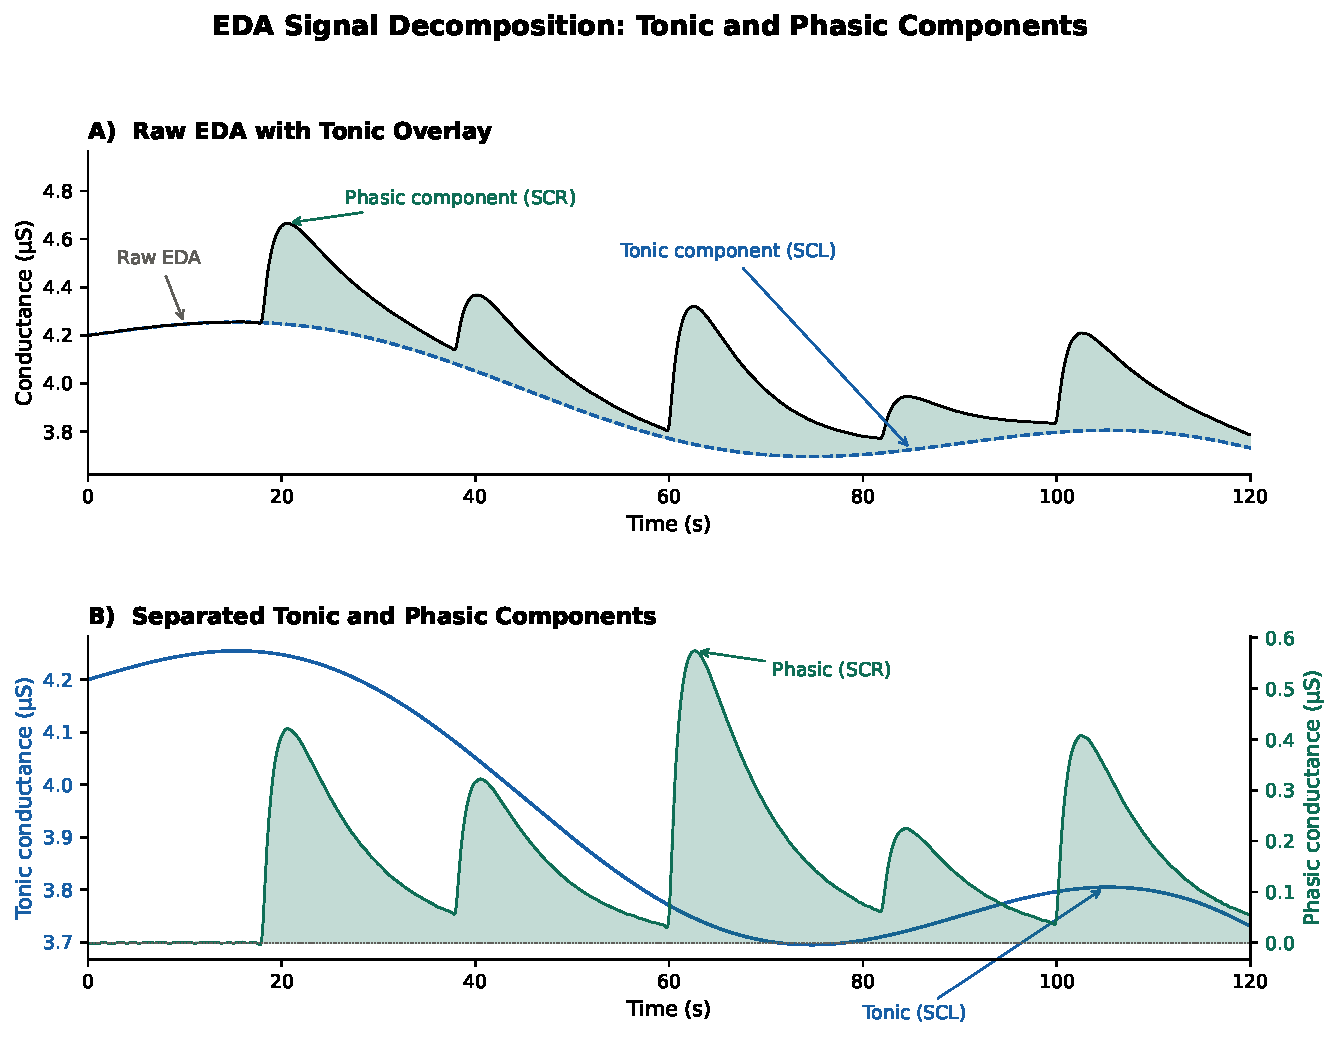
\includegraphics[width=\textwidth]{figures/eda_tonic_phasic.pdf}
    \caption{%
    Decomposition of a synthetic \gls{eda} signal into its tonic and phasic components.
    \textbf{A)} The raw \gls{eda} signal (black) with the tonic component (\gls{scl}, blue dashed) overlaid. Phasic activity above the tonic baseline is shaded green.
    \textbf{B)} The tonic and phasic components are shown separately. The tonic component reflects slow baseline drift in skin conductance, while the phasic component captures stimulus-evoked \glspl{scr} superimposed on that baseline.
    Synthetic data for illustration.}
    \label{fig:eda_signal_decomp}
\end{figure}

\FloatBarrier
\subsection{Measurement Techniques} \label{sec:EDA_measurement}

% Endosomatic vs exosomatic; scope narrowed to exosomatic
\Gls{eda} is measured either without externally applied current (endosomatic) or with an external source (exosomatic). Endosomatic measurements record the potential difference between an active (palmar) and an inactive (bony reference) site on the skin. Exosomatic measurements apply an external \gls{dc} or \gls{ac} source through electrodes and measure the resulting voltage or current to derive skin conductance, impedance, or admittance~\cite{boucsein_electrodermal_2012, tronstad_current_2022}. Endosomatic responses are difficult to parameterize, and endosomatic recordings measure skin potential rather than skin conductance. Most contemporary \gls{eda} devices therefore use exosomatic techniques~\cite{boucsein_electrodermal_2012, posada-quintero_innovations_2020}.


\subsubsection{Exosomatic DC Recording} \label{sec:EDA_DC}
% Exosomatic recording DC (Physical quantities: Skin conductance/resistance - Why DC? Not only because of AC clashes with EMG measurements, but maybe from a psychological viewpoint - Refer to Pabst AC vs DC EDA in methodology)
% DC recording: popularity, three-factor rationale, excitation standards, literature compatibility
Exosomatic \gls{dc} recording with a constant-voltage source is the most widely used method in electrodermal research~\cite{boucsein_electrodermal_2012, posada-quintero_innovations_2020}. Its popularity reflects three advantages. First, the instrumentation is simple, requiring only a constant \gls{dc} voltage and an \gls{opamp} front end. Second, the measurement uses only two electrodes, and the conductance derivation assumes a single return path for the excitation current, through the skin between the two electrodes~\cite{boucsein_electrodermal_2012}. Third, a single skin conductance channel carries both the tonic \gls{scl} and the phasic \glspl{scr}~\cite{gersak_electrodermal_2020, zangroniz_electrodermal_2017, tronstad_current_2022}. The standard excitation level is the constant voltage applied across the skin to drive the measurement current. It is \qty{0.5}{\volt} or, equivalently, a constant current below \SI{10}{\micro\ampere\per\centi\meter\squared}~\cite{boucsein_electrodermal_2012}. Constant voltage dominates by convention, as it produces skin conductance directly without transformation~\cite{boucsein_electrodermal_2012}. Most \gls{eda} studies have used this method, so its psychological correlates are well established and results are directly comparable across the existing literature~\cite{boucsein_electrodermal_2012, posada-quintero_innovations_2020}.

% DC disadvantages: polarization, drift, non-linearities
The main disadvantage of \gls{dc} excitation is electrode polarization, which generates counter-\gls{emf} at the electrode-skin interface and can corrupt the \gls{eda} signal even when using Ag/AgCl (silver/silver-chloride) electrodes, the EDA-recording standard for low drift and biocompatibility~\cite{posada-quintero_innovations_2020, boucsein_electrodermal_2012}. These effects worsen in long-term recordings and contribute to baseline drift~\cite{pabst_comparison_2017}. At excitation voltages above approximately \qty{0.8}{\volt} across a single recording site, non-linearities appear in the current-voltage relationship and distort the measured conductance value~\cite{pabst_comparison_2017, boucsein_electrodermal_2012}. The Methods chapter sets the EDA front-end excitation conditions accordingly (Section~\ref{sec:EDA_current_source}).

\subsubsection{Exosomatic AC Recording} \label{sec:EDA_AC}
% Exosomatic recording AC (Physical quantities: Impedance, Phase, and Capacitance - Skin admittance or skin impedance)
% Write more about what info the AC recording gives us?

% AC admittance definition
Exosomatic \gls{ac} recording applies a small sinusoidal voltage or current at a constant frequency and measures the resulting skin admittance or impedance. The admittance is complex, with an in-phase conductance component and an out-of-phase susceptance component~\cite{boucsein_electrodermal_2012, tronstad_current_2022}.

% AC advantages: reduced polarization and access to susceptance and endogenous SP
\Gls{ac} recording reduces electrode polarization and counter-\gls{emf}, because the alternating polarity prevents the sustained interface charging that develops under \gls{dc} excitation~\cite{pabst_comparison_2017, posada-quintero_innovations_2020}. It also recovers the susceptance component of the skin admittance and supports simultaneous endogenous \gls{sp} measurement on the same electrodes~\cite{pabst_comparison_2017}.

% AC disadvantages: instrumentation complexity, no standard, frequency-band interference
\Gls{ac} recording has three disadvantages. First, \gls{ac} devices require complex instrumentation, including constant-amplitude \gls{ac} generation and phase-sensitive rectification, to decompose the admittance into its conductance and susceptance components. Second, the field has not established a standard technique for \gls{ac} recording~\cite{boucsein_electrodermal_2012}. Third, interference at the \gls{ac} excitation frequency cannot be separated from the \gls{eda} signal. \gls{dc} recording avoids this, because the \gls{eda} signal occupies the \qtyrange{0}{1.5}{\hertz} band and any interference above it can be removed by low-pass filtering~\cite{boucsein_electrodermal_2012}.

% DC chosen for this thesis, hand-off to methods

\textcite{martinsen_sources_2015} suggested excitation frequencies in the range \qtyrange{10}{20}{\hertz} for \gls{ac} exosomatic recording. This range falls inside the \gls{semg} bandwidth established in Section~\ref{sec:sEMG} (\qtyrange{10}{500}{\hertz}) and would be indistinguishable from the sEMG signal. This thesis therefore uses \gls{dc} exosomatic recording. The design of the \gls{dc} acquisition circuit is presented in Section~\ref{sec:EDA_frontend}.

\subsection{Electrode Placement and Sites}\label{sec:eda_electrode_sites}

Palmar recording sites are conventional in \gls{eda} measurement because the eccrine sweat glands of the palm are densely innervated by sympathetic fibers and respond reliably to arousal stimuli~\cite{boucsein_electrodermal_2012, tronstad_current_2022}. The hypothenar eminence at the muscular base of the little finger and the thenar eminence at the muscular base of the thumb are established palmar sites for \gls{eda} recording~\cite{boucsein_electrodermal_2012, tronstad_current_2022}. The electrode placement used in this thesis is described in Section~\ref{sec:electrode_placement}.


\section{Ground Loop} \label{sec:ground_loops}
% EMG Ref electrode corrupts the EDA current path
% Section pipeline: Generic ground loop definition → Biopotential + bioimpedance co-measurement scenario → Galvanic isolation as solution (hand-off to methods sec:galvanic_isolation).
% Chapter role: Supplies the theoretical foundation that methods sec:galvanic_isolation cites directly. Grounds the two-corruption-path framing (injected current diversion + biopotential voltage drop) that justifies the ISO224 isolation choice and predicts the Q6 validation result.

%1. Definition of Ground Loop  
% Generic definition of ground loop
In electrical measurements, all voltages are referenced to a common ground point. A ground loop forms when a circuit contains more than one conductive path to that ground, which allows unintended currents to circulate through the loop. These circulating currents appear as noise or bias in the recorded signal~\cite{kamen_essentials_2010}.

%2. How It Arises in Biopotential Measurements
% Specific case: biopotential + bioimpedance co-measurement on the same subject
Ground loops become a direct measurement concern when two instruments are connected to the same subject~\cite{webster_medical_2020}. A biopotential instrument records a voltage generated by tissue at the electrode without applying any excitation, while a bioimpedance instrument injects a known excitation and characterizes the tissue from the response~\cite{grimnes_bioimpedance_2015}. Consider the case where one instrument measures a biopotential and uses a ground electrode on the subject, while a second instrument injects a small current into the subject to measure its bioimpedance. If the two instruments share a common ground, the injected current finds a second return path through the first instrument's reference electrode instead of returning through the bioimpedance-measurement path~\cite{huhta_60-hz_1973}. The biopotential measurement can be affected because the diverted current induces a voltage drop across any impedance in the shared ground path. The diverted current also reduces the current through the measurement path, corrupting the bioimpedance reading.

The two-instrument case applies to this thesis. The \gls{eda} front-end injects an excitation current, and the \gls{emg} front-end uses a ground electrode in galvanic contact with the body. The \gls{dc} exosomatic conductance measurement described in Section~\ref{sec:EDA_DC} assumes a single return path for the excitation current, and the shared-ground configuration violates that assumption. At the \gls{eda} injection electrode (where the excitation current enters the skin), Kirchhoff's current law gives

\begin{equation}
I_{R_{\text{ref}}} = I_{\text{skin}} + I_{\text{parasitic}},
\label{eq:kcl_eda_active}
\end{equation}

where $I_{\text{skin}}$ returns through $R_{\text{skin}}$ to the \gls{eda} return electrode and $I_{\text{parasitic}}$ returns through $R_{\text{parasitic}}$ to the \gls{emg} ground electrode. $R_{\text{parasitic}}$ is the impedance of the body-side path from the \gls{eda} injection electrode to the \gls{emg} ground electrode contact. It exists because the \gls{emg} ground electrode shares a ground node with the \gls{eda} return electrode under the shared-ground configuration. $R_{\text{parasitic}}$ cannot be predicted from circuit specifications alone. The two return paths sit in parallel between the \gls{eda} injection electrode and the shared ground node, so the \gls{eda} front-end measures an effective skin resistance equal to the parallel combination of the two paths,

\begin{equation}
R_{\text{measured}} = \frac{R_{\text{skin}} \, R_{\text{parasitic}}}{R_{\text{skin}} + R_{\text{parasitic}}},
\label{eq:r_measured}
\end{equation}

instead of $R_{\text{skin}}$ alone. The shared-ground configuration is the conductive route that galvanic isolation removes.

%3. Galvanic Isolation as the Solution
% Galvanic isolation as the solution
\subsubsection{Galvanic Isolation}
\label{sec:galvanic_isolation_theory}

Galvanic isolation removes the conductive path between two circuit domains while preserving signal or power transfer across the boundary. On the primary side, the source circuit operates from its own ground reference. On the secondary side, the destination circuit operates from a separate ground reference. The two sides share no direct conductor and exchange information through capacitive, magnetic, or optical coupling~\cite{webster_medical_2020}. Each coupling type has its own bandwidth, isolation rating, and power-handling envelope.

The two coupling mechanisms relevant to this thesis are capacitive and magnetic isolation. Capacitive isolation passes a differential analog signal across a non-conductive barrier between primary and secondary domains. This non-conductive boundary is the isolation barrier referenced in subsequent chapters. The barrier supports the bandwidths required for biopotential and bioimpedance recording while maintaining a high isolation rating~\cite{webster_medical_2020}. Magnetic isolation routes power through a transformer winding instead of a shared conductor. The transformer suits power transfer because the secondary side delivers continuous current without a shared ground return.


Galvanic isolation eliminates the conductive return path described in the preceding paragraphs. After isolation, \gls{eda} and \gls{emg} acquisition no longer share a ground reference, so the \gls{eda} excitation current cannot divert through the \gls{emg} ground electrode. The parallel-paths effect captured by Equation~\ref{eq:r_measured} is therefore removed~\cite{kusche_galvanically_2017}. The implementation is described in Section~\ref{sec:galvanic_isolation}.



\begin{comment}
    
\begin{itemize}
    \item You need a background to present your results
    \item Often based on standard textbooks and key articles in your field
    \item Make sure you present it in your context
    \item Be aware of plagiarism traps
    \item Don't go back to year 0
\end{itemize}
\end{comment}